\documentclass{../../tex_template/asaproc}
\usepackage{graphicx} % \includegraphics
\usepackage{float}    % To keep figures in right place. 
                      % Usage: \being{figure}[H] \includegraphics{tmp.pdf} \end{figure}
\usepackage{subfig}   % \subfloat
\usepackage{amsmath}  % bmatrix, pmatrix, etc
\usepackage{bm}
\newcommand{\p}[1]{\left(#1\right)}
\newcommand{\bk}[1]{\left[#1\right]}
\newcommand{\bc}[1]{ \left\{#1\right\} }
\newcommand{\abs}[1]{ \left|#1\right| }
\newcommand{\norm}[1]{ \left|\left|#1\right|\right| }
\newcommand{\E}{ \text{E} }
\newcommand{\N}{ \mathcal N }
\newcommand{\ds}{ \displaystyle }

%\usepackage{times}
%If you have times installed on your system, please
%uncomment the line above

%For figures and tables to stretch across two columns
%use \begin{figure*} \end{figure*} and
%\begin{table*}\end{table*}
% please place figures & tables as close as possible
% to text references

\newcommand{\be}{\begin{equation}}
\newcommand{\ee}{\end{equation}}
\newcommand{\y}{\bm y}
\newcommand{\X}{\bm X}

\title{Quiz 2 --- EU referendum poll tracker}

%input all authors' names
\author{
  Arthur Lui$^1$\\
  University California -- Santa Cruz$^1$\\
}

%input affiliations
%{USDA Forest Service Forest Products Laboratory}

\begin{document}
\maketitle
\begin{abstract}
Members of the European Union (EU) are concerned about the sentiments of the
British people on whether the UK should remain in the EU. As of this point, the
opinions are fairly evenly split. The people of the UK will vote on a
referendum on 23 June, 2016. The majority vote will decide the outcome.
Clearly, the outcome will affect not only the UK but countries in the EU, and
other concerned countries around the world, as the EU is not only a a group of
countries that trade freely with one another but also a symbol of unity among
nations arisen after World War II. Consequently, many policy makers and
researchers are interested in modeling the outcome of the vote. Currently, the
sentiment of the British people are captured by different polls which are
conducted through different medium (phone / internet).  But certain methods
introduce bias. It is, therefore, the task of this paper to determine the
effect of different polling methods on sentiment. Moreover, since the data
provided by BBC has been recorded since September 2015 at regular time
intervals till the present day, the effect of time is also examined. A Bayesian
Lasso regression model is used for this study to aid in variable selection.
\begin{keywords}
Lasso, Bayesian lasso, EU, regression, phone / online polls bias.
\end{keywords}
\end{abstract}

\section{Introduction}
Modeling the effect of different polls that record the sentiment of the EU
referendum voters is of interest to policy makers, world leaders, business
owners, UK citizens, and many others. Many polls and polling methods currently
exist to measure sentiment. People's preference can also change over time.
Consequently, a model that incorporates time and polling method should be used
in such an analysis. In addition, since many variables exist when considering a
model that accounts for different polling methods, using some type of variable
selection mechanism helps to produce simpler and more interpretable models.
In this paper, the model used will be a Bayesian lasso regression model.
The outcome of interest is the proportion of voters in favor of leaving the
EU (of the people that have a preference). This is computed as the number
of people in favor of leaving over the sum of the number of people
in favor of leaving and the number of people in favor of remaining within
a given time period. Note that the number of people that don't have a preference
are not included in computing the proportion. We will call this proportion 
$p$. However, directly modeling $p$ is problematic as its value is constrained
to be between 0 and 1. So instead, the logit of $p$ is modeled. We let logit($p$)
be $y$. We have 100 such data points from September 2015 to May 2016. The model
was trained with only half of the data (selected at random in R using a seed of 207).
To model the temporal trend, I created a predictor of lag 1 of the outcome
variable $y$. (So, I now have only 99 observations to use.) The different 
pollsters (1) Survation, (2) ICM, (3) Opinium, (4) YouGov, (5) ComRes, (6)Ipsos Mori,
(7) TNS, (8) BMG, and (9) Panelbase, are used as covariates. There are
only two mediums for administering the surveys in the data -- by (a) phone
and (b) internet. Figure \ref{fig:pairs} shows the scatter plot matrix of
the data described above. Some clear observations can be made. (1) Temporal 
trends, if they exist, do not appear to be strong. (2) There is perhaps 
a strong correlation between the polling method and voter preference.
\begin{figure}[H]
  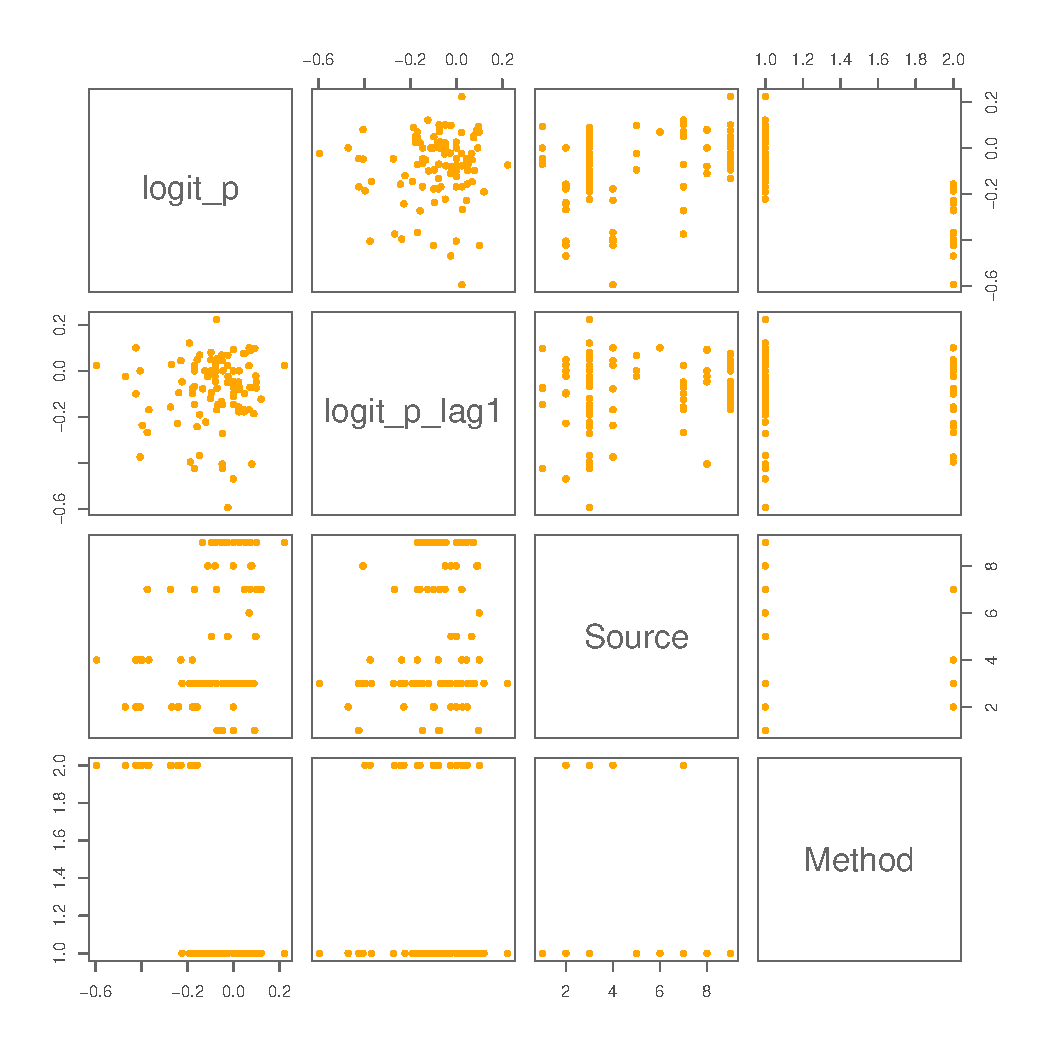
\includegraphics[scale=.5]{figs/pairs.pdf}
  \caption{\small Scatter plot matrix of (1) logit($p$), where $p$ is the
    number of people in favor of leaving the EU over the sum of the number of
    people in favor of leaving the EU and the number of people in favor of
    remaining in the EU; (2) logit(p) with a lag of 1 time period; (3) Survey
    Source which is one of Survation, ICM, Opinium, YouGov, ComRes, Ipsos Mori,
    TNS, BMG, or Panelbase; (4) Surveying Method: Phone or Online.}
  \label{fig:pairs}
\end{figure}

\section{Methods}
Here, we focus on the methods for the analysis. The model of choice here is a
Bayesian lasso model. In my opinion, a multiple linear regression model without
a variable selection may have been suitable as well. From past experience, when
the true model actually contains many variables, using a lasso model may not be
ideal. But here, I think it is rather clear from the data that not all
variables are important in predicting the outcome. So, implementing a lasso
model may help to simply the model by shrinking unimportant variables to 0,
achieving model selection. \\

Park and Casella (2008) outline the details for a Bayesian implementation of
the lasso by Tibshirani and Brieman. The core idea in (frequentist) lasso is
that a penalty term is introduced for large covariate values while optimizing a
linear model. This idea is embodied by the following expression
\[
  \text{argmax}_\beta \p{ \norm{\y - \X\bm\beta}^2 +\lambda\sum_{j=1}^J{\beta_j^2}},
\]
where $J$ is the number of covariates.  Here, $\lambda$ is a tuning parameter
which is often learned using cross validation.\\

In the Bayesian implementation, the following hierarchical representation for the model
is suggested
\[
\begin{array}{rclcl}
  \y &|& \mu,\X,\bm\beta,\sigma^2 &\sim& \text{N}_n(\mu\bm1_n + \X\bm\beta, \sigma^2 \bm I_n) \\
  \bm\beta &|& \sigma^2,\tau^2_1,...,\tau^2_J &\sim& \text{N}_J(\bm 0_J, \sigma^2\bm D_\tau), \\
           &&&& \bm D_\tau  = \text{diag}(\tau^2_1,...,\tau^2_J)\\
           &&p(\sigma^2,\tau^2_1,...,\tau^2_p) &\propto& \pi(\sigma^2) \prod_{j=1}^J 
  \frac{\lambda^2}{2}  e^{-\lambda^2\tau_j^2/2},\\
\end{array}
\]
where $\y$ and $\X$ are the centered and scaled response and predictors
respectively.  $\lambda$ and $\tau_j^2$ are auxiliary variables which simplify
the computation so that Gibbs steps can be implemented to avoid metropolis
steps. The resulting full conditionals are as follows:
\[
\begin{array}{rclcl}
  \bm\beta &|& ... &\sim& \text{N}_J(A^{-1}\X^{T}\y,\sigma^2A^{-1})\\
           &&&& \text{where } A = \X^{T}\X + D_\tau^{-1}\\
  \sigma^2 &|& ... &\sim& \text{IG}((n-1)/2+p/2,\\
           &&&&\quad\norm{\y-\X\bm\beta}^2+\bm\beta^T\bm D^{-1}_\tau\bm\beta/2)\\
  \frac{1}{\tau_j} &|&... &\sim& \text{Inverse-Gaussian}(\sqrt\frac{\lambda^2\sigma^2}{\beta_j^2},\lambda^2)
\end{array}
\]
In addition, a hyper prior can be placed on $\lambda^2$ so that cross
validation can be avoided to select $\lambda^2$. A suitable choice for a prior
for $\lambda^2$ is a Gamma prior with shape $r$ and rate $\delta$. The
resulting full conditional for $\lambda^2$ is a Gamma distribution with shape
$J+r$ and rate $\sum_{j=1}^J\tau_j^2+\delta$. For this problem, I selected
$r=1$ and $\delta=1.5$ so that the prior is relatively uninformative.\\

This completes the model specification and the full conditionals are all in closed
form, which means a fully Gibbs implementation can be used.\\

In this analysis, only half of the data (selected at random) were used to fit the
model. The remaining half are used as testing data.\\

%The parameter $\mu$ is given a flat prior and is integrated out to simplify computation.
%Treat $\sigma^2$ as 1 here because the columns are standardized. Also, treat $\mu$ as 0 because columns are centered.

\section{Analysis}

The Gibbs sampler was implemented with 100000 iterations as burn in and 2000
samples were used for the remaining analysis. Figure \ref{fig:allposts} shows
the posterior means and their 95\% HPD's for all the covariates. 
%Note that the intercept is not included here because the covariates and response were centered and scaled. 
These are the posteriors for the coefficients of the centered and scaled covariates. 
\begin{figure}[H]
  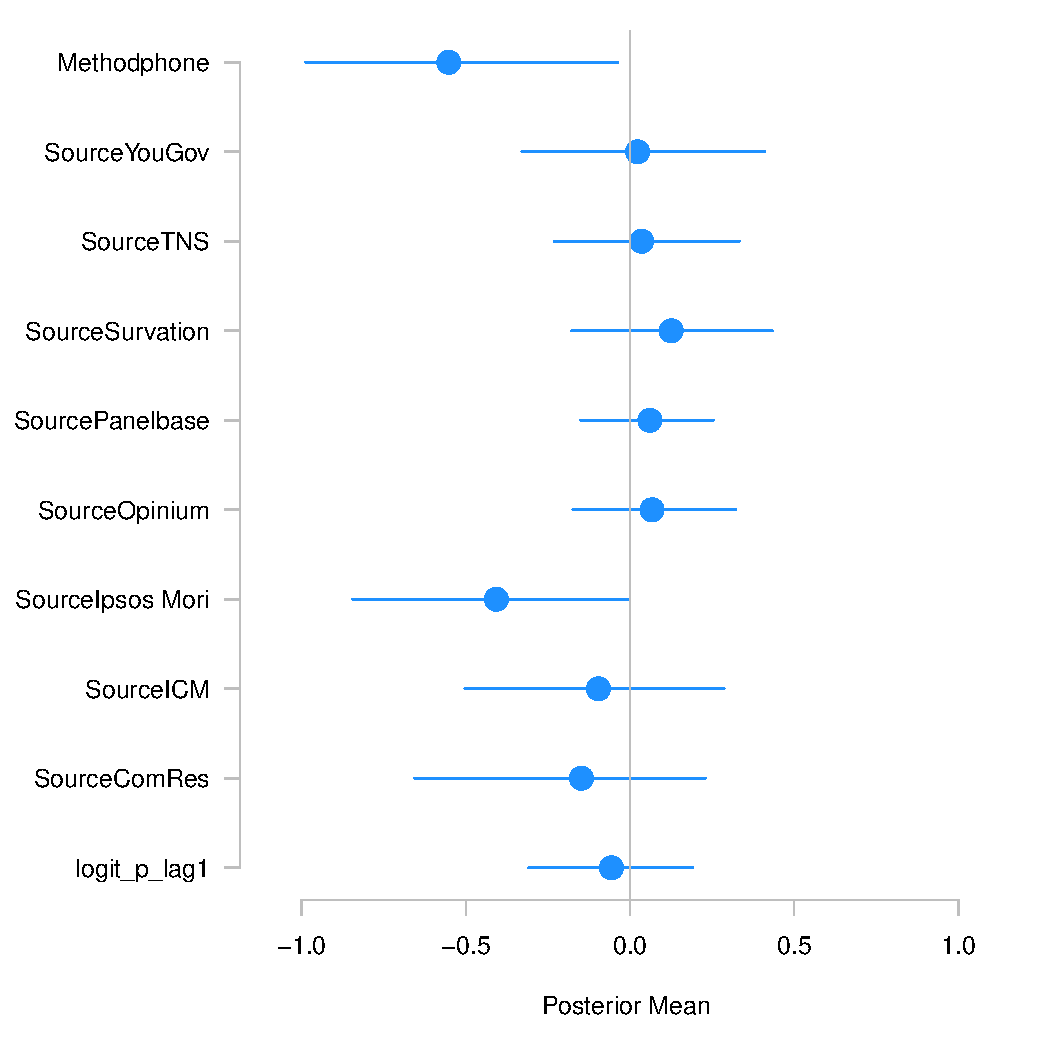
\includegraphics[scale=.5]{figs/allposts.pdf}
  \caption{\small The posterior means and 95\% HPD's for each covariate coefficient.
  Phone surveys from Ipsos Mori appear to be associated with negative outcomes (i.e.
  lower proportion of people in favor of leaving the EU.)}
  \label{fig:allposts}
\end{figure}
Observe that as expected, the method of surveying appears to have a strong effect on
the outcome. Phone surveys are associated with a negative outcome (i.e. a lesser
proportion of people in favor of leaving the EU). The pollster Ipsos Mori
appears to be associated with a negative outcome as well. All the other variables 
are shrunk to 0. Figure \ref{fig:posts} shows the posterior distributions of
only the covariate associated with Ipsos Mori pollster and the coefficient for
phone surveys.
\begin{figure}[H]
  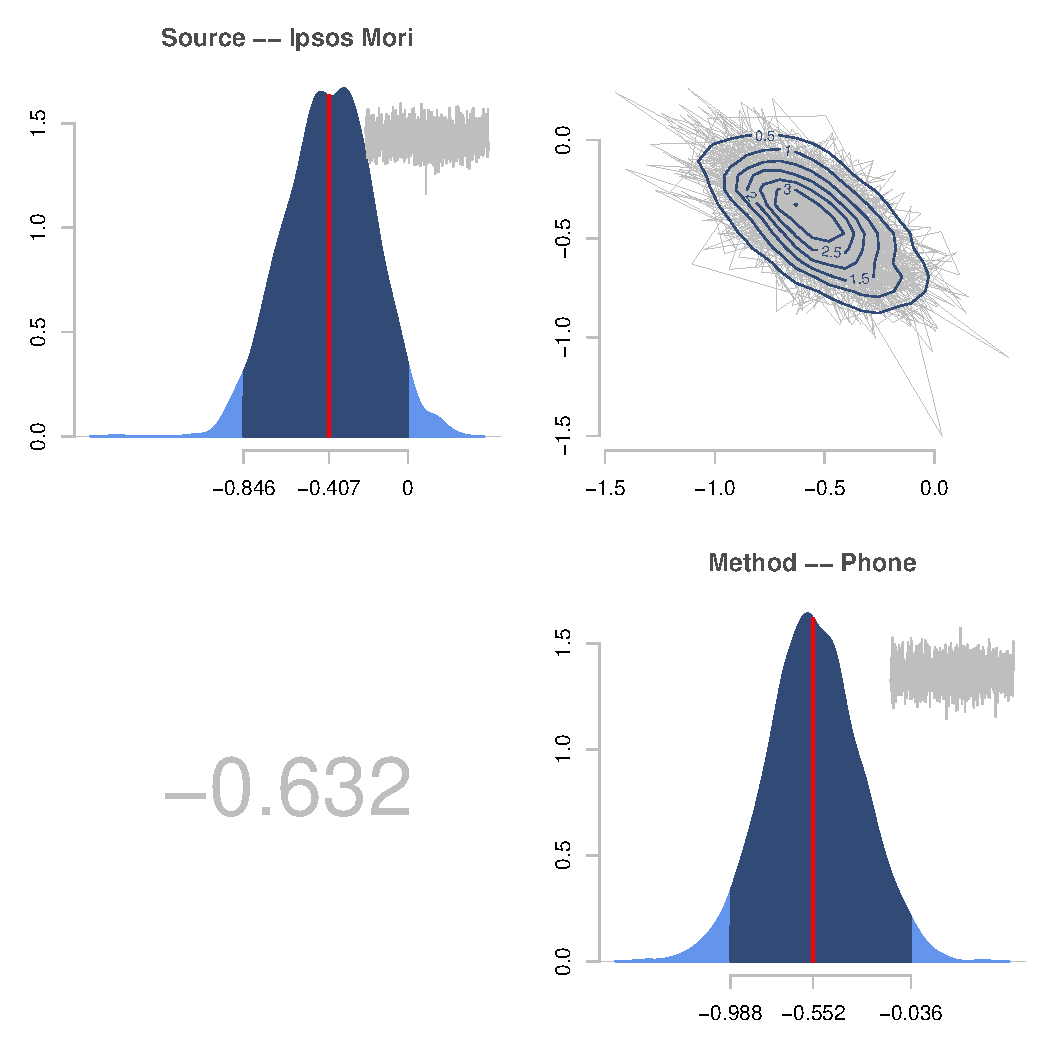
\includegraphics[scale=.5]{figs/posts.pdf}
  \caption{\small Posterior distributions for Ipsos Mori coefficient and Phone survey coefficient.
  They are negatively correlated and are the only 2 variables which are far away from 0. Their
  posterior means (red line) and their 95\% HPD's (navy blue region) are negative. The trace plots 
  for the distributions indicate there is no strong evidence against non-convergence.}
  \label{fig:posts}
\end{figure}
The posterior mean for the coefficient associated with phone surveys is -.552
and they posterior mean for the coefficients associated with Ipsos Mori source
is -.407.\\

Now we answer the questions of interest. (1) There is in fact no temporal trend
observed from this model. The posterior mean for the coefficient for the lag-1
variable is close to 0 (-.0565). The 95\% credible interval contains 0. This 
suggests that over time, opinions are not changing dramatically.
(2) There are differences in the various pollster sources. The Ipsos Mori poll is
associated with lower outcomes. None of the other sources seem to strongly
affect the outcome. This could be the case because people with different political
preferences tend to access certain pollsters more frequently. This is an item
that warrants further investigation. (3) Phone polls are associated with lower outcomes.
This could be the case because of an interviewer effect. Perhaps people are not as
honest when they report their preferences over the phone. Again, this is another
item that warrants further investigation.\\

Finally, we use the test data assess the predictive strength of the model used.
In Figure \ref{fig:preds}, the posterior predictive means evaluated at the
testing data. Note that the covariates were first uncentered and unscaled.
Then the predictions were obtained and the inverse logit was taken.  The data
were partitioned and color-coded into 4 groups: (1) Ipsos Mori phone surveys
(red), (2) non-Ipsos-Mori phone surveys (blue), (3) Ipsos Mori online surveys
(green), and (4) non-Ipsos-Mori online surveys (orange).  Note that there are
in fact no Ipsos Mori online surveys. Therefore, an interaction effect should
have been included in the model. This is an item to note for a future study.
\begin{figure}[H]
  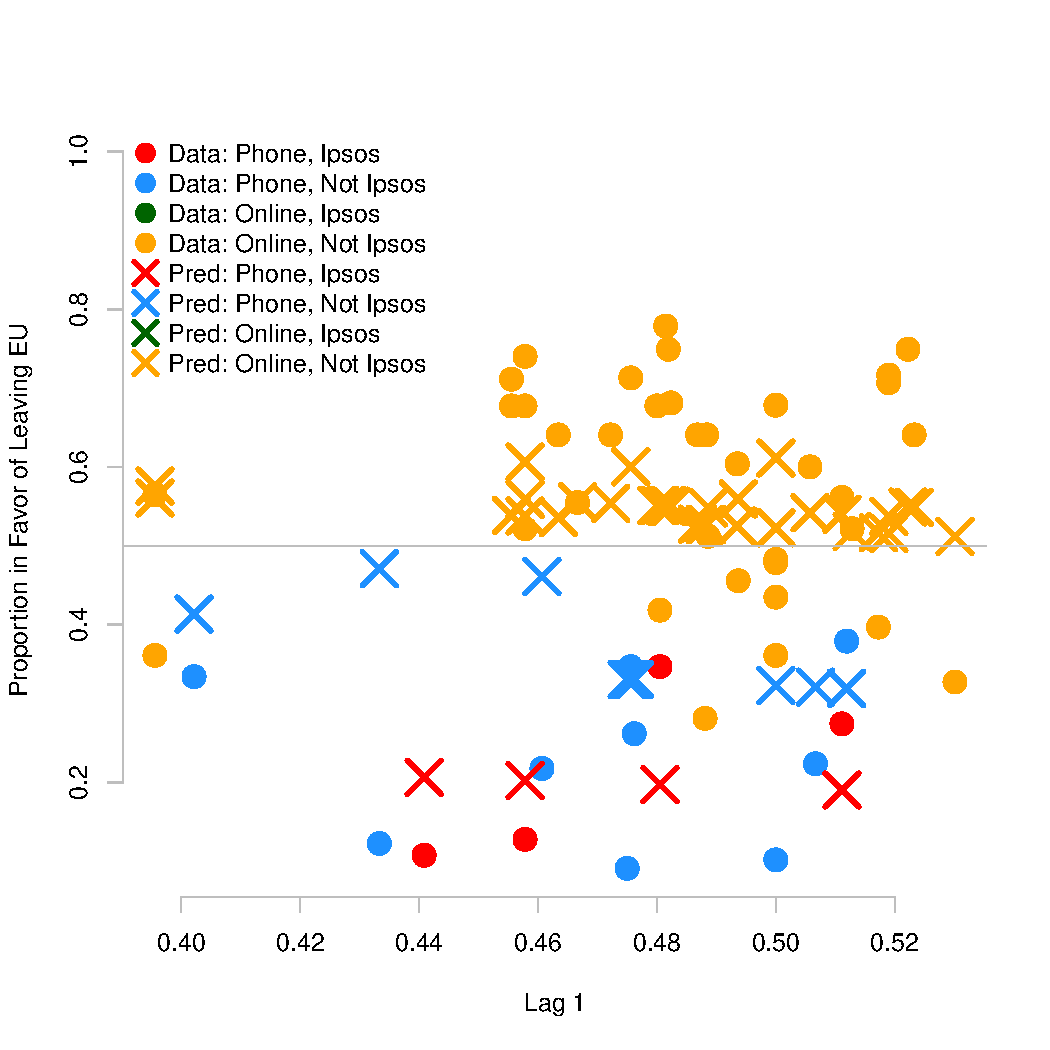
\includegraphics[scale=.5]{figs/preds.pdf}
  \caption{\small I used all the $\beta$'s because it was easier. I don't think it matters since the other regressors are shrunk to 0.}
  \label{fig:preds}
\end{figure}
Visually observe that the predictions follow the general pattern of the data
moderately well (the colors match). We can further see that non-Ipsos-More
online surveys are associated with higher outcomes. The predicted proportion of
people in favor of leaving the EU is lower for the non-Ipsos-Mori phone
surveys. That of the Ipsos-Mori phone surveys are the lowest.

\section{Conclusions}
A Bayesian lasso model was fit to the EU data. No temporal trends were
discovered. Poll sources indeed have some association with lower proportions of
people in favor of remaining in the EU (for the Ipsos Mori source). Phone
surveys are associated with lower proportions as well. Why this is the case is
unclear, and warrants further investigation.  Though there may be confounding
in phone surveys because people may be reluctant to tell discuss their true
preferences. Online surveys promote anonymity. Pollsters may be confounded by
the political preferences of the voter. Last of all, there are no voters who
used Ipsos online surveys. This could be the case because there may be no Ipsos
online surveys available, but only phone surveys. A new model involving an
interaction term for Ipsos phone surveys should be included.

\begin{references}
{\footnotesize
\itemsep=3pt
\item {\em Park, T., \& Casella, G. (2008). The bayesian lasso. Journal of the American Statistical Association, 103(482), 681-686.}
\item {\em Gelman, A., Carlin, J. B., Stern, H. S., \& Rubin, D. B. (2014). Bayesian data analysis (Vol. 2). Boca Raton, FL, USA: Chapman \& Hall/CRC, 73.}
}

\end{references}
\end{document}

%\begin{figure*}
%  \centering
%  \includegraphics[scale=.55]{figs/mapDat.pdf}
%  \vspace{-7em}
%  \caption{\small Some Caption.}
%  \label{fig:mapDat}
%\end{figure*}

%\begin{figure}[H]
%  \includegraphics[scale=.5]{figs/pairsLogRate.pdf}
%  \caption{\small Hi Motor vehicle theft is not strongly correlated with any other thefts.}
%  \label{fig:logOdds}
%\end{figure}
